\documentclass{beamer}
\beamertemplatenavigationsymbolsempty
\usetheme{Ilmenau}
\usecolortheme{beaver}
%\usepackage[utf8]{inputenc}
\usepackage[english]{babel}
\parindent=0.pt
\usepackage{amsmath}
\usepackage{graphicx}
\usepackage{verbatim}
\usepackage{tikz}
\usepackage{csquotes}
\usepackage[backend=biber,
style=phys,
citestyle=authoryear
]{biblatex}
\addbibresource{biblio.bib} 
\usepackage[export]{adjustbox}
\usefonttheme[onlymath]{serif}
\newcommand{\R}{\mathbb{R}}
\renewcommand{\qedsymbol}{\includegraphics[width=0.6in, right]{QED Gregory.png}}


\title{Thermodynamic Costs of Turing Machines \parencite{Kolchinsky_2020}}
\author{Daniel Briseno}

  \begin{document}
  \frame{\titlepage}
  
  
%%%%%%%%%%%%%%%%%% Paper intro %%%%%%%%%%%%%%

\begin{frame}{Context of the Paper}
\begin{block}{Prior work on Thermodynamics of Information Processing}
\begin{itemize}
    \item Landauer cost of erasing a bit: $kT\ln2$ (1961)
    \item Logically reversible computations can be performed with no heat or entropy production (1973)
    \item Informal argument for minimum cost of $x\mapsto y$ (1989 - 2019)
    \item Development of non-equilibrium statistical physics
    \begin{itemize}
        \item Trajectory-based and stochastic thermodynamics (2013-2015)
    \end{itemize}
    \item Thermodynamic costs of specific implementations of Turing Machines (TM)(2015-2019)
    
    
\end{itemize}
\end{block}
\end{frame}


  \begin{frame}{Purpose of the Paper}
    \begin{block}{Thermodynamic costs of computation}
    \begin{itemize}
        \item Extends results to general class of TM
        \item Analyzes the thermodynamic costs of $f:\mathbb{N} \nrightarrow \mathbb{N}$ on a physical implementation of a TM $M$
        \item Logical properties of $f$ and $M$ impose constraints on thermodynamic costs.
        \item Result might generalize to any implementation of a TM
    \end{itemize}
    \end{block}
\end{frame}

%%%%%%%%%%%%%%%%%%%%%% CS Background %%%%%%%%%%%%%%%%%%%%%%
\begin{frame}{CS Background}
    \begin{block}{Turing Machines}
        \begin{figure}
            \centering
            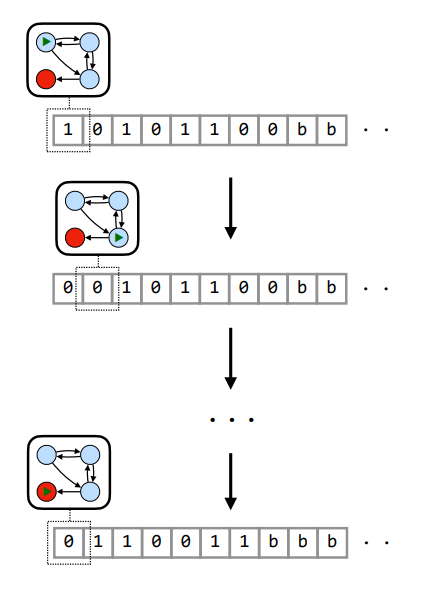
\includegraphics[height=5cm]{TM.png}
            \caption{Graphical representation of a TM}
            \label{fig:my_label}
        \end{figure}
    \end{block}
\end{frame}

\begin{frame}{CS Background}
\begin{block}{Turing Machines}
Formal definition of a Turing Machine:
    \begin{itemize}
        \item A Turing machine $M$ is a 4-tuple $M = (Q,\Sigma, q_0,\delta) $ where:
        \begin{itemize}
            \item $Q$ is a finite nonempty set of states.
            \item $\Sigma$ is a finite nonempty set of symbols.
            \item $q_0\in Q$ is the initial state of $M$
            \item $\delta: (Q\times \Sigma) \nrightarrow (\Sigma \times \{L,R\}\times Q)$ is a partial transition function determining the symbol written on the tape, the movement of the read-write head, and the next state of the $M$.
        \end{itemize}
    \end{itemize}
\end{block}
\end{frame}

\begin{frame}{CS Background}
    \begin{block}{Additional Assumptions on TM $M$}
    
    \begin{enumerate}
        \item $\Sigma = \{0,1,b\}$
        \item If and when $M$ halts on an input, the tape will contain an output string $s\in \{0,1\}^*$ followed by all blank symbols, and the pointer will be set to the start of the tape.
    \end{enumerate}
    Assumptions do not affect the computational capabilities of $M$.
    \end{block}
\end{frame}
    
\begin{frame}{CS Background}
    \begin{block}{Turing Machines as Partial Functions}
    Any computation performed by a TM $M$ can be represented as
    \begin{equation*}
        \phi_M:\{0,1\}^* \nrightarrow \{0,1\}^*
    \end{equation*}
    and $\phi_M(x) = y$ indicates that $M$ started with input program $x$ yields the output string $y$.
    \end{block}
    \begin{block}{Universal TM}
    There exist Universal Turing Machines (UTM) such that given a UTM $U$ and any TM $M$, there exists an interpreter program $\sigma_{U,M}$ such that
    \begin{equation*}
        \phi_U(\sigma_{U,M},x) = \phi_M(x)
    \end{equation*}
    \end{block}
\end{frame}

\begin{frame}{CS Background}
    \begin{block}{Computability}
    \begin{itemize}
        \item Church Turing Thesis: A function can be calculated by a sequence of formal operations if and only if it is computable by a Turing Machine.
       \item Physical Church Turing Thesis: Any function implemented by a physical process can also be implemented by a Turing Machine
    \end{itemize}
    \end{block}
\end{frame}



%%%%%%%%%%%%%%%%%%%%%%%%%%%%%%%%%% Realization of a TM%%%%%%%%%%%%%%%%%%
\begin{frame}{Realizations of a TM}
    \begin{block}{Realizations and Computable Realizations}
    \begin{itemize}
        \item \textbf{Physical Realization}: A physical process consistent with the laws of thermodynamics and whose dynamics correspond to the input-output map of a TM $M$
        \item \textbf{Computable Realization}: A physical realization of a TM $M$ whose generated heat on an input program $x$ can be determined by a computable function
    \end{itemize}
    \end{block}
\end{frame}

%%%%%%%%%%%%%%%%%%%%%%%%%% AIT Background %%%%%%%%%%%%%%%%%%%%%%%%%%%%%%%
\begin{frame}{Algorithmic Information Theory}
\begin{block}{Kolmogorov Complexity}
The Kolmogorov complexity $K_U$ of a bitstring $x$ is the length of the shortest input program that when given to a UTM $U$ can produce $x$ as an output:
\begin{equation*}
    K_U(x) :=\min_{z:\phi_U(z) = x}\ell(z)
\end{equation*}
\begin{itemize}
    \item Measure of amount of information in $x$
\end{itemize}
\end{block}
\end{frame}

\begin{frame}{Algorithmic Information Theory}
    \begin{block}{Kolmogorov Complexity of Bitstring $x$}
    \begin{equation*}
        K_U(x) :=\min_{z:\phi_U(z) = x}\ell(z)
    \end{equation*}
    \end{block}
    \begin{block}{Kolmogorov Complexity of a Computable Function $f$}
    \begin{equation*}
        K_U(f) := \min_{M:\phi_M = f} \ell(\sigma_{U,M})
    \end{equation*}
    \end{block}
    \begin{block}{Conditional Kolmogorov Complexity of $x$ Given Bitstring $y$}
\begin{equation*}
    K_U(x|y) = \min_{z:\phi_U(z,y) = x} \ell(z)
\end{equation*}
\end{block}
\end{frame}

\begin{frame}{Algorithmic Information Theory}
    \begin{block}{Invariance Theorem}
    For distinct UTM $U$, $U'$:
        \begin{equation*}
            K_{U'}(x) = K_U(x) + O(1)
        \end{equation*}
        Thus, $U$ is usually omitted and we write $K(x)$ for Kolmogorov complexity of $x$
    \end{block}
\end{frame}

\begin{frame}{Algorithmic Information Theory}
\begin{block}{Incompressible string $x$}
If $x$ is incompressible, then 
\begin{equation*}
    K(x) = \ell(\text{print }x)
\end{equation*}
\begin{itemize}
    \item Any program capable of producing $x$ must contain $x$ explicitly
    \item $x$ is ``maximally dense" with information
\end{itemize}
\end{block}
 \begin{block}{Highly compressible string $\pi$}
    \begin{equation*}
        K(\pi) \le \ell \left( 6\sin^{-1}\left(\frac{1}{2}\right)\right) < \ell( \text{print }\pi)
    \end{equation*}
    \end{block}
\end{frame}

\begin{frame}{Algorithmic Information Theory}
\begin{block}{Input Distributions}
\begin{itemize}
    \item Input string $x$ as random variable with probability distribution $p_X$
    \item Important example: coin flipping distribution of TM $M$
    \begin{equation*}
        m_X^\text{coin}(x) := \begin{cases} 2^{-\ell(x)} &\text{if $x\;\in$ dom $\phi_M$}\\ 0 &\text{otherwise}\end{cases}
    \end{equation*}
    \item With normalizing constant $\Omega_M :=\sum_{x\in\text{ dom }\phi_M} 2^{-\ell(x)}$
    \begin{equation*}
        p_X^\text{coin}(x) = m_X^\text{coin}(x)/\Omega_M
    \end{equation*}
\end{itemize}
\end{block}
\end{frame}

\begin{frame}{Algorithmic Information Theory}
    \begin{block}{Shannon Entropy of Distribution $p_X$}
    \begin{equation*}
    S(p_X) = - \sum_{x\in X} p_X(x)\ln p_X(x)    
    \end{equation*}
    \begin{itemize}
        \item Measure of amount of information in $p_X$
        \item $\ln \frac{1}{p_X}$: "surprisal``, how unexpected, and hence informative, is $x$?
        \item $p_X(x)$: how often do we receive surprise $\ln p_X$
    \end{itemize}
    \end{block}
\end{frame}

\begin{frame}{Algorithmic Information Theory}
    \begin{block}{Entropy Production (EP)}
    The expected EP, written $\Sigma (p_X)$ of a physical process with initial state distribution $p_X$ and final state distribution $p_Y$ is:
    \begin{align*}
        \Sigma (p_X) &= S(p_Y) - S(p_X) + \langle Q \rangle_{p_X}/kT
    \end{align*}
    Thermodynamically reversible processes have $\Sigma (p_X)=0$. EP is always nonnegative.
    \end{block}
\end{frame}

\begin{frame}{Physical Setup}
\begin{block}{System under consideration}
The authors consider a physical system which:
\begin{itemize}
    \item has a countable state-space $\mathcal{X}$
    \item is connected to a work reservoir and a heat bath at temperature $T$. The bath is taken to be in a Boltzmann distribution.
    \item evolves according to a driving protocol in the time interval $[0,t_f]$.
\end{itemize}
In this scenario, the heat function $Q(x)$ is defined as the expected amount of heat transferred from the system to the heat bath assuming that the system began in state $x$.
\end{block}
\end{frame}

\begin{frame}{Physical Setup}

    \begin{figure}
            \centering
            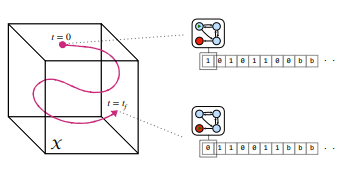
\includegraphics{System.png}
            \label{fig:my_label2}
        \end{figure}
\end{frame}

\begin{frame}{Physical Setup}
\begin{block}{System under consideration}
The joint Hamiltonian of the system is
\begin{equation*}
    H_X^t(x) + H_B(b) + H_{\text{int}}(x,b)
\end{equation*}
If $p_B(b)$ is the initial distribution of the bath and $p'_{B|X}$ is the final distribution, then $Q(x)$ is more formally defined as:
\begin{equation*}
    Q(x) = \langle H_B \rangle_{p'_{B|x}} - \langle H_B \rangle_{p_B}
\end{equation*}
\end{block}
\end{frame}

\begin{frame}{Physical Setup}
    \begin{block}{Realization Formally Defined}
    A physical process is a \textbf{realization} of a partial function $f:\mathcal{X}\nrightarrow\mathcal{X}$ if the conditional probability of the system's final state given the initial state follows:
    \begin{equation*}
        p_{Y|X}(y|x) = \delta(f(x), y)
    \end{equation*}
    \end{block}
    
\begin{block}{Realization of a TM Defined}
\begin{itemize}
    \item Recall that a TM $M$ can be written as a partial function $\phi_M:\{0,1\} \nrightarrow \{0,1\}$
    \item A physical process is a realization of a TM $M$ if it is a realization of $\phi_M$.
\end{itemize}
\end{block}
\end{frame}


%%%%%%%%%%%%%%%%%%%%%%%%%%%%%%% Proposition 1 %%%%%%%%%%%%%%%%%%%%%%%%%%
\begin{frame}{Prop. 1}

\begin{block}{Proposition 1}
Given a countable set $\mathcal{X}$ and partial functions $f:\mathcal{X} \nrightarrow \mathcal{X}$ and $G:\mathcal{X} \nrightarrow \mathbb{R}$, the following are equivalent:
\begin{enumerate}
    \item For all $p_X$ with $\text{supp}\: p_X \subseteq \text{dom}\: f$
    \begin{equation*}
        \langle G \rangle_{p_X} + S[p_{f(X)}] - S(p_X) \ge 0
    \end{equation*}
    \item For all $y\in \text{img}\: f$
    \begin{equation*}
        \sum_{x:f(x) = y} e^{-G(x)} \le 1
    \end{equation*}
    \item There exists a realization of $f$ coupled to a heat bath at temperature $T$ whose heat function $Q$ obeys
    \begin{align*}
        Q(x)/kT &= G(x)  &&\forall x\in\text{dom}\:f
    \end{align*}
\end{enumerate}
\end{block}
\end{frame}


\begin{frame}{Prop.1 As Generalization of Landauer Cost}

Take $x\in\{0,1\}$ to be a random bit determined by a coin toss, and $f$ as the bit-erasing operation $f(x) = 0$. Then:
\begin{align*}
    p_X(x) &= \frac{1}{2}\\
    p_{f(X)}(y) &= \begin{cases} 0 &\text{if } y=1\\ 1 &\text{if }y=0\end{cases}
\end{align*}
Then for any $G(x) = Q(x)/kT$, condition 1 implies:
\begin{align*}
    \langle G \rangle_{p_X} + S[p_{f(X)}] - S(p_X) &\ge 0\\
    \implies \langle G\rangle_{p_X} &\ge S(p_X)\\
    \implies \langle G\rangle_{p_X} &\ge \ln 2
\end{align*}
\end{frame}

\begin{frame}{Prop.1 As Generalization of Landauer Cost}
We would like to characterize the cost of an arbitrary bit deletion, so taking $G$ to be identical for inputs $\{0,1\}$
\begin{align*}
    G(x) \ge \ln 2
\end{align*}
and using equivalent condition 3 from Proposition 1 we recover the Landauer cost of a bit deletion:
\begin{align*}
    Q(x)/kT &\ge \ln 2\\
    \implies Q(x) \ge kT \ln 2
\end{align*}
\end{frame}

%%%%%%%%%%%%%%%%%%%%%%%%%%%%%%%%% Realizations of a TM %%%%%%%%%%%%%%%%%%%%%%%%%

\begin{frame}{Realizations of TM}
\begin{block}{Realizations of TM Used in Analysis}
    \begin{itemize}
        \item \textbf{Coin-Flipping Realization}: thermodynamically reversible when inputs are sampled from coin-flipping distribution
        \item \textbf{Dominating Realization}: produces less heat than any computable realization of a TM
    \end{itemize}
\end{block}
\end{frame}




%%%%%%%%%%%%%%%%%%%%%%%%%%%%%%%%%%%% Coin-Flipping Analysis %%%%%%%%%%%%%%%%%%%%%%%%%%%
\begin{frame}{Coin-Flipping Realization}
    \begin{block}{Input Distribution}
     \begin{equation*}
        m_X^\text{coin}(x) := \begin{cases} 2^{-\ell(x)} &\text{if $x\;\in$ dom $\phi_M$}\\ 0 &\text{otherwise}\end{cases}
    \end{equation*}
    \begin{equation*}
        p_X^\text{coin}(x) = m_X^\text{coin}(x)/\Omega_M
    \end{equation*}
    \end{block}
    \begin{block}{Output Distribution}
    \begin{equation*}
        m_Y^\text{coin}(y) = \sum_{x:\phi_M(x) = y} 2^{-\ell(x)}
    \end{equation*}
    \begin{equation*}
        p_Y^\text{coin}(y) = m_Y(y) / \Omega_M
    \end{equation*}
    \end{block}
\end{frame}


\begin{frame}{Coin-Flipping Realization}
\begin{block}{Associated Heat Function of Coin-Flipping Realization for TM $M$}
Can be shown that 
\begin{equation*}
    G(x) = -\ln p_X^\text{coin}(x) + \ln p_Y^\text{coin}[\phi_M(x)]
\end{equation*}
Satisfies  condition 2 of Prop 1. Thus, multiplying by $kT$ and using definitions of $p_X^\text{coin}$ and $p_Y^\text{coin}$:
\begin{align*}
    Q_\text{coin}(x) &= kT\{-\ln p_X^\text{coin} (x)+ \ln p_Y^\text{coin}[\phi_M(x)]\}\\
    &= kT\ln \{\ell(x) + \log_2 m_Y[\phi_M(x)]\}
\end{align*}
\end{block}
\end{frame}

\begin{frame}{Coin-Flipping Realization}
    \begin{block}{Zero Entropy Production}
    \begin{equation*}
        Q_\text{coin}(x) = kT\{-\ln p_X^\text{coin} + \ln p_Y^\text{coin}[\phi_M(x)]\}
    \end{equation*}
    Using 
    \begin{equation*}
        \langle Q_\text{coin} \rangle_{p_X}=\sum_{x\in X}p_X(x)Q(x)
    \end{equation*}
    We can verify that:
    \begin{align*}
        &\langle Q_\text{coin}\rangle_{p_X} = kT\{ S(p_X^\text{coin}) - S(p_Y^\text{coin})\}\\
        \implies &\Sigma(p_X^\text{coin}) = S(p_Y^\text{coin}) - S(p_X^\text{coin}) + S(p_X^\text{coin}) - S(p_Y^\text{coin}) = 0
    \end{align*}
    \end{block}
\end{frame}

\begin{frame}{Coin-Flipping Realization}
\begin{block}{Associated Heat Function of Coin-Flipping Realization for TM $M$}
\begin{equation*}
    Q_\text{coin}(x) = kT\ln \{\ell(x) + \log_2 m_Y[\phi_M(x)]\}
\end{equation*}
Recall definition of $m_Y$:
\begin{equation*}
        m_Y^\text{coin}(y) = \sum_{x:\phi_M(x) = y} 2^{-\ell(x)}
    \end{equation*}
\begin{itemize}
    \item $\log_2 m_Y[\phi_M(x)]$ minimal for logically reversible $\phi_M$.
    \item $Q_\text{coin}$ minimal for short and logically reversible input programs.
\end{itemize}
\end{block}
\end{frame}

\begin{frame}{Coin-Flipping Realization}
    \begin{block}{Levin's Coding Theorem for UTM}
    \begin{align*}
        -\log_2 m_Y(y) = K(y) + O(1)
    \end{align*}
    \end{block}
    \begin{block}{Heat Function for UTM}
    \begin{equation*}
        Q_\text{coin}(x) = kT\ln 2 \{\ell(x) - K[\phi_M(x)]\} + O(1)
    \end{equation*}
    \begin{itemize}
        \item $Q_\text{coin}$ achieves its minimum value when $x$ is the shortest program capable of producing $\phi_U(x)$ (always true if $\phi_U$ is reversible).
        \begin{equation*}
            \min_{x:\phi_U(x)=y} Q_\text{coin}(x) = O(1)
        \end{equation*}
    \end{itemize}
    \end{block}
\end{frame}

\begin{frame}{Coin-Flipping Realization}
\begin{block}{Expected Heat of Coin-Flipping Distribution}
Recall that 
\begin{equation*}
    \langle Q_\text{coin}\rangle_{p_X} = kT\{ S(p_X^\text{coin}) - S(p_Y^\text{coin})\}
\end{equation*}
\begin{itemize}
    \item Difference of entropies is infinite
    \item Implies infinite expected heat
    \item Implies infinite expected length of input programs and infinite expected runtime
\end{itemize}
\end{block}
\end{frame}

\begin{frame}{Coin-Flipping Realization}
    \begin{block}{Initial Distribution for Minimum Expected Heat}
    Input distribution can be varied to minimize $Q(x)$ in a UTM:
    \begin{align*}
        p_X^\text{min} (x)&= \delta(x_0,x)\\
        Q_\text{coin}(x_0) &= \min_{x\in X} Q(x) = O(1)\\
        \langle Q_\text{coin}\rangle_{p_X^\text{min}} &= O(1)
    \end{align*}
    But then EP is no longer 0:
    \begin{equation*}
        \Sigma(p_X^\text{min}) = S(p_Y^\text{min}) - S(p_X^\text{min}) + O(1) > 0
    \end{equation*}
    \end{block}
\end{frame}

%%%%%%%%%%%%%%%%%%%%%%%%%%%%% Analysis of Dominating Realization %%%%%%%%%%%%%%%%%%%%%%%

\begin{frame}{Dominating Realization}
\begin{block}{Heat Function for Dominating Realization of TM $M$}
Can be shown that $G(x) = \ln 2K[x|\phi_M(x)]$ satisfies condition 2 of Prop 1. Thus
\begin{equation*}
    Q_\text{dom} = kT\ln 2K[x|\phi_M(x)]
\end{equation*}
is the heat function for a realization, called the \textit{dominating realization}, of TM $M$.
\begin{itemize}
    \item Inputs generating a lot of heat are large and incompressible, and $\phi_M$ is non-invertible for that input
    \item Inputs generating little heat are those for which $\phi_M$ is invertible
    \begin{itemize}
        \item For these inputs, $Q(x) = O(1)$
    \end{itemize}
\end{itemize}
\end{block}
\end{frame}

\begin{frame}{Dominating Realization}
\begin{block}{Non-Computability}
    \begin{itemize}
        \item Dominating realization is not computable
        \item It is upper semi-computable
        \begin{itemize}
            \item Can be obtained in limit by sequence of increasingly efficient computable realizations $Q_n(x)$
            \item Converges on $Q_\text{dom}(x)$ from above
        \end{itemize}
    \end{itemize}
    \end{block}
\end{frame}

\begin{frame}{Dominating Realization}
\begin{block}{Efficiency of Dominating Realization}
    $Q_\text{dom}$ is optimal in the sense that for any other \textit{computable} realization with heat function $Q(X)$:
    \begin{align*}
        Q(x) \ge Q_\text{dom} - kT[\ln 2K(Q/kT) + K(\phi_M)] + O(1)
    \end{align*}
    \begin{itemize}
        \item $Q_\text{dom}$ is minimal up to a negative constant. 
        \begin{itemize}
            \item For $Q(x) \le Q_\text{dom}$, $\phi_M$ has to have high complexity, or $Q$ has to have high complexity
        \end{itemize}
        \item The above inequality only holds true for computable realizations. Thus it is not necessarily true that $Q_\text{dom}\le Q_\text{coin} + O(1)$
    \end{itemize}
\end{block}
\end{frame}


%%%%%%%%%%%%%%%%%%%%%%%%%%%%%%%%%%% Heat vs Complexity Trade-off %%%%%%%%%%%%%%%%%%%%%%%%%

\begin{frame}{Dominating Realization}
\begin{block}{Heat VS. Complexity Trade-off}
     \begin{equation*}
        Q(x) \ge Q_\text{dom} - kT[\ln 2K(Q/kT) + K(\phi_M)] + O(1)
    \end{equation*}
    Using $Q_\text{dom} = kT\ln 2K[x|\phi_M(x)]$ and re-arraigning gives:
    \begin{equation*}
        Q(x)/\ln 2 + K(Q) + K(f) \ge K(x|y) + O(1)
    \end{equation*}
    \begin{itemize}
        \item Every computation mapping $x$ to $y$ comes with a "cost`` of $K(x|y)$
        \item Cost can be paid by generating heat, having a high complexity heat function, or having a high complexity mapping $f$
    \end{itemize}
\end{block}
\end{frame}

\begin{frame}{Heat Vs. Complexity Trade-off}

    \begin{figure}
            \centering
            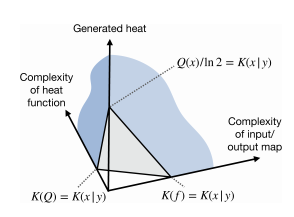
\includegraphics{HeatvsComplexity.png}
            \label{fig:my_label1}
        \end{figure}
    
\end{frame}


\begin{frame}{Heat VS. Complexity Trade-off}
    \begin{block}{Example: Erasing a Bitstring}
    \begin{equation*}
        Q(x)/\ln 2 + K(Q) + K(f) \ge K(x|y) + O(1)
    \end{equation*}
    \begin{itemize}
        \item Consider the an example where $f$ erases a long and incompressible bitstring $x$.
        \item $x\mapsto y$ comes with an intrinsic cost of $K(x|y) = K(x) \approx \ell(x)$
    \end{itemize}
    \end{block}
\end{frame}


\begin{frame}{Heat VS. Complexity Trade-off}
    \begin{block}{Generate a Lot of Heat}
    Take $f$ to be
    \begin{equation*}
        f(x') = `000...000' \:\forall x'
    \end{equation*}
    \begin{itemize}
        \item $f$ has low complexity
        \item Using dominating implementation, $Q(x)/\ln 2 = K(x|y) = K(x)\approx \ell(x)$
        \begin{itemize}
            \item Heat function has low complexity
            \item $x$ long and incompressible implies high heat generation
        \end{itemize}
    \end{itemize}
    \end{block}
\end{frame}

\begin{frame}{Heat Vs. Complexity Trade-off}
\begin{block}{Have a High Complexity Heat Function}
Can be shown that the following heat function satisfies conditions of Prop.1 for dominating realization of $f(x') = `000...000'$
\begin{equation*}
    Q(x') := \begin{cases} Q_\text{dom}(x') &x'\not\in \{x,`000...000'\}\\
    Q_\text{dom}(`000...000') &x' =x\\
    Q_\text{dom}(x) &x' = `000...000'\end{cases}
\end{equation*}
\begin{itemize}
    \item Generates little heat
    \item Low complexity $f$
    \item $x$ hard-coded into $Q$ implies high complexity heat function
\end{itemize}
\end{block}
\end{frame}

\begin{frame}{Heat Vs. Complexity Trade-off}
\begin{block}{Have a High Complexity Mapping}
Consider the logically reversible map:
\begin{equation*}
    f(x') := \begin{cases} x' & x\not\in \{x,`000...000'\}\\
    `000...000' & x=x'\\
    x & x'= `000...000'\end{cases}
\end{equation*}
\begin{itemize}
    \item Logically reversible maps can be carried out with 0 heat generation
    \item 0 heat generation would imply minimally complex heat map
    \item $x$ hard-coded into $f$ implies high complexity mapping
\end{itemize}
\end{block}
\end{frame}

\begin{frame}{Physical Church-Turing Thesis}
\begin{block}{Significance of Physical Church Turing Thesis}
\begin{itemize}
    \item Current conclusions only apply to computable realizations
    \item In principle, non-computable realizations of TM could exist 
    \item Validity of Church-Turing Thesis would imply any physical realization of a TM must follow thermodynamic constraints shown in paper
\end{itemize}
\end{block}
\end{frame}


\begin{frame}{Conclusion}

\begin{itemize}
    \item Proposition 1 allows us to relate logical properties of a TM to its thermodynamic properties.
    \item Coin-flipping realization gives a highly thermodynamically reversible case
    \begin{itemize}
        \item Infinite expected heat for zero EP input distribution
        \item Heat minimizing input distribution implies nonzero EP
    \end{itemize}
    \item Dominating realization gives lower bound on heat production for any computable realization
    \begin{itemize}
        \item Upper semicomputable
        \item The inequality $ Q(x)/\ln 2 + K(Q) + K(f) \ge K(x|y) + O(1)$ allows us to decompose intrinsic cost of mapping $x\mapsto y$ into complexity of heat function, complexity of mapping, and heat production.
    \end{itemize}
\end{itemize}

\end{frame}

\begin{frame}{References}
    \printbibliography
\end{frame}


\end{document}